\subsubsection{Llargada del formulari}

\paragraph{}
Aquesta funcionalitat pot arribar a presentar un formulari relativament llarg si considerem tots els camps, en teoria disponibles, de cara a la cerca de persones. Per aquest motiu, s'han dissenyat un parell de funcionalitats que pretenen facilitar la comprensió i utilització del formulari de cerca.

La primera d'elles, és que els blocs del formulari referents a la persona cercada i els seus relatius més propers, poden ser contrets i expandits, mitjançant un clic en la capçalera del bloc.

Per tal d'indicar que es pot interactuar amb aquestes capçaleres, s'ha afegit el signe `-' o `+', a l'esquerra del títol i una icona que també reflecteix l'estat actual, del bloc del formulari, a la dreta. A la vegada, un text en cursiva explica la funcionalitat en la mateixa barra i el color de la barra, canvia en passar el ratolí per sobre i la icona es transforma en una mà d'interacció.

La segona funcionalitat, té l'objectiu de facilitar la iniciació de la cerca. En moltes circumstàncies, els usuaris només voldran emplenar detalls bàsics de la persona principal a cercar i no pas dels seus relatius. En aquestes situacions, sobretot en dispositius mòbils, el botó de cercar quedarà molt allunyat de l'inici del formulari i per tant, pot resultar confús pels usuaris com iniciar la cerca.

Per evitar aquesta confusió, un cop se superen 780 píxels de la posició inicial del formulari de la persona principal i fins que s'arriba a la posició original del botó de cerca, una barra fixa apareix al final de la pàgina amb el botó de cercar i se sobreposa al contingut de la pàgina web. D'aquesta forma, el botó de cercar és accessible en tot moment pels usuaris, sense necessitat d'arribar al final del formulari.

La figura~\ref{fig:interactiveFormBloc} mostra els dos estats possibles, de les capçaleres dels blocs del formulari i la barra mencionada, que apareix sobre impressionada al final de la pantalla amb el botó de cerca, quan es compleixen les condicions necessàries.

\begin{figure}
    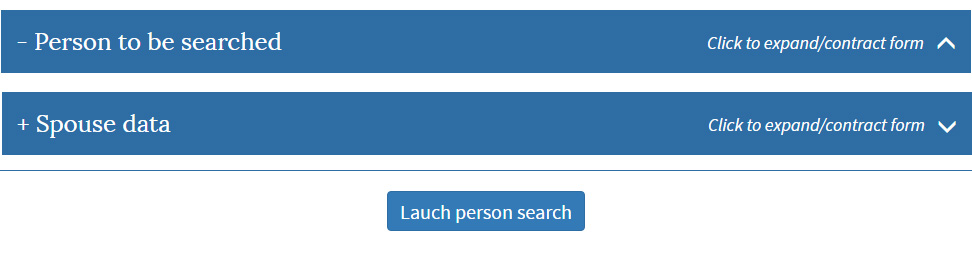
\includegraphics[width=\linewidth]{11/02_searchPersons/03_formBars}
    \centering
    \caption{Blocs de formulari interactius i sobreposició del botó de cerca}\label{fig:interactiveFormBloc}
\end{figure}

L'efecte de la barra sobre impressionada amb el botó de cerca, s'aconsegueix mitjançant jQuery i el canvi de classes CSS, en els elements HTML que contenen la barra de cerca. El jQuery s'encarrega d'espiar la posició de l'usuari cada cop que es desplaça verticalment per la pàgina web i les diferents classes CSS, fixen o alliberen, la posició del contenidor de la barra de cerca.

A continuació, mostrem la classe CSS que converteix la barra de cerca, en una barra de posició fixa, al final de la pàgina web. Les propietats que ho fan possible son la propietat, \emph{position:fixed} i \emph{bottom:0px}.

\begin{lstlisting}[style=rawOwn,caption={Classe CSS per sobre impressionar el botó de cerca}]
.detached-bottom {
    position: fixed;
    bottom: 0px;
    height: 80px;
    width: 100%;
    margin-top: 0px;
    border-top: 1px solid #2e6da4;
    z-index: 9999;
    background-color: #fff;
    -webkit-transition: all 0.2s linear;
    -moz-transition: all 0.2s linear;
    -o-transition: all 0.2s linear;
    transition: all 0.2s linear;
}
\end{lstlisting}
